\documentclass[a4paper]{article}
\usepackage{url,verbatim,fancyvrb}
\usepackage{pifont}
% \usepackage[latin1]{inputenc}
\usepackage[pdftex]{graphicx}
\usepackage[authoryear]{natbib}
\usepackage{color,gretl}
\usepackage[letterpaper,body={6.3in,9.15in},top=.8in,left=1.1in]{geometry}
\usepackage[pdftex,hyperfootnotes=false]{hyperref}
\usepackage{amsmath,bm}
\usepackage[bottom]{footmisc}

\begin{document}

% \newcommand{\obsvec}{\mathbf{y}}
% \newcommand{\obsmat}{\mathbf{H}}
% \newcommand{\obsx}{\mathbf{x}}
% \newcommand{\obsxmat}{\mathbf{A}}
% \newcommand{\obsdist}{\mathbf{w}}
% \newcommand{\obsvar}{\mathbf{R}}

% \newcommand{\statevec}{\bm{\xi}}
% \newcommand{\statevar}{\mathbf{P}}
% \newcommand{\statemat}{\mathbf{F}}
% \newcommand{\strdist}{\mathbf{v}}
% \newcommand{\strvar}{\mathbf{Q}}
% \newcommand{\gain}{\mathbf{K}}
% \newcommand{\statemu}{\bm{\mu}}

% \newcommand{\altstrvar}{\mathbf{B}}
% \newcommand{\altobsvar}{\mathbf{C}}
% \newcommand{\alldist}{\bm{\varepsilon}}

% \newcommand{\prederr}{\mathbf{e}}
% \newcommand{\predvar}{\bm{\Sigma}}

% less fussy?
\newcommand{\obsvec}{y}
\newcommand{\obsmat}{H}
\newcommand{\obsx}{x}
\newcommand{\obsxmat}{A}
\newcommand{\obsdist}{w}
\newcommand{\obsvar}{R}

\newcommand{\statevec}{\alpha}
\newcommand{\statevar}{P}
\newcommand{\statemat}{F}
\newcommand{\strdist}{v}
\newcommand{\strvar}{Q}
\newcommand{\gain}{K}
\newcommand{\statemu}{\mu}

\newcommand{\altstrvar}{B}
\newcommand{\altobsvar}{C}
\newcommand{\alldist}{\varepsilon}

\newcommand{\prederr}{e}
\newcommand{\predvar}{\Sigma}
% end less fussy

\newcommand{\myvec}{\mbox{vec}}
\newcommand{\myvech}{\mbox{vech}}

\makeatletter
\def\pdots{\vbox{\baselineskip2.5\p@ 
  \lineskiplimit\z@ \kern2\p@\hbox{.}\hbox{.}\hbox{.}\hbox{.}}}
\makeatother

\setlength{\parindent}{0pt}
\setlength{\parskip}{1ex}

\title{State Space Modeling in gretl:\\a revised interface}
\author{Allin Cottrell and Riccardo ``Jack'' Lucchetti}
\maketitle

\section{Introduction}
\label{sec:amble}

The original interface to the treatment of linear state space models
in gretl predated the development of gretl's ``bundle'' type. It
recently struck the gretl authors that the bundle type could be used
to advantage in reformulating the user interface; we suspect people
will find the new interface a good deal easier to use. Moreover, the
new interface makes it much more practical to split long portions of
code into smaller, dedicated functions, which are arguably easier to
debug and maintain; this should hopefully lead to more function
packages using gretl's native state space facilities.

In general, a gretl bundle is an all-purpose container into which you
can put matrices, scalars, strings and so on, identified by keys. A
Kalman bundle is a somewhat regimented version of the same. There are
two sets of ``reserved'' keys, one set pertaining to input matrices
and the other to results generated by the Kalman functions.  Beyond
that, however, you are free to add to the bundle whatever extra
elements you think may be useful.

Here are the main features of the new interface ``at a glance'':
%
\begin{itemize}
\item The Kalman structure, which used to be entirely \textit{sui
    generis}, is implemented as a bundle.
\item You can therefore have as many named models as you like in
  existence at one time, and you can pass them as arguments to
  functions.
\item The ``block'' syntax for defining a filter is replaced by the
  function \cmd{ksetup}.
\item The signatures of the functions \cmd{kfilter} and \cmd{ksmooth}
  are much simplified. For the most part you retrieve results by
  reading bundle members instead of poking in matrix-pointer
  arguments.
\item A new function, \cmd{kdsmooth}, implements Koopman's
  ``disturbance smoother.''
\item The \cmd{ksimul} function has been revamped and improved.
\end{itemize}

At present the old syntax and methods, as described in chapter 30 of
the \textit{Gretl User's Guide}, are still available, with the new
interface operating in parallel. However, we may retire the old
interface at some point. Please note that you cannot ``mix and match''
the old and new interfaces; you must adhere consistently to one or the
other.

\section{Notation}

As a reminder, the basic representation of a state-space model as
given in the \textit{Gretl User's Guide} is as follows:
%
\begin{align}
  \label{eq:state}
  \statevec_{t+1} &= \statemat_t \statevec_t + \strdist_t \\
  \label{eq:obs}
  \obsvec_t &= \obsxmat_t'\obsx_t + \obsmat_t' \statevec_t +
  \obsdist_t 
\end{align}
%
where (\ref{eq:state}) is the state transition equation and
(\ref{eq:obs}) is the observation or measurement equation.  The state
vector, $\statevec_{t}$, is ($r \times 1$) and the vector of
observables, $\obsvec_t$, is ($n \times 1$); $\obsx_t$ is a ($k
\times 1$) vector of exogenous variables.  The ($r \times 1$) vector
$\strdist_t$ and the ($n \times 1$) vector $\obsdist_t$ are assumed to
be vector white noise:
%
\begin{align*}
E(\strdist_t \strdist_s') &= \strvar_t \mbox{ for } t = s, 
    \mbox{ otherwise } \mathbf{0} \\
E(\obsdist_t \obsdist_s') &= \obsvar_t \mbox{ for } t = s, 
    \mbox{ otherwise } \mathbf{0}
\end{align*}

The number of time-series observations is denoted by $T$.  In the case
when $\statemat_t = \statemat$, $\obsmat_t = \obsmat$,
$\obsxmat_t = \obsxmat$, $\strvar_t = \strvar$ and
$\obsvar_t = \obsvar$ for all $t$, the model is said to be
\emph{time-invariant}. We assume time-invariance in most of what
follows, but discuss the time-varying case in
section~\ref{sec:tvarying}.

\section{Defining the model}
\label{sec:setup}

The \cmd{ksetup} function is used to initialize a state space
model, by specifying only its indispensable elements: the observables
and their link to the unobserved state vector, plus the law of motion
for the latter and the covariance matrix of its
innovations. Therefore, the function takes a minimum of four
arguments.\footnote{An optional, fifth argument is used for
  initializing a state space model in which there is some non-zero
  correlation between $\strdist_t$ and $\obsdist_t$. See section
  \ref{sec:crossd}.} The corresponding bundle keys are as follows:

\begin{center}
\begin{tabular}{ccl}
Symbol & Dimensions & Reserved key \\[6pt]
$\obsvec$      & $T \times n$ & \texttt{obsy}\\
$\obsmat$      & $r \times n$ & \texttt{obsymat}\\
$\statemat$    & $r \times r$ & \texttt{statemat}\\
$\strvar$      & $r \times r$ & \texttt{statevar}\\
\end{tabular}
\end{center}

For example,
\begin{code}
bundle SSmod = ksetup(y, H, F, Q)
\end{code} 

The names of these input matrices don't matter; in fact they may be
anonymous matrices constructed on the fly. But if and when you wish to
copy them out of the bundle, you must use the specified keys:
\begin{code}
matrix H = SSmod.obsymat
\end{code}

Although all the arguments are in concept matrices, as a convenience
you may give \texttt{obsy} as a series or list of series, and the
other arguments can be given as scalars if in context they are
$1 \times 1$.

An important detail: from the user's point of view, the bundle created
by \cmd{ksetup} looks like any other user-created bundle. However,
bundles created via \cmd{ksetup} contain quite a few hidden,
read-only elements that are essential for the whole apparatus to work.

If applicable you may specify any of the following optional input
matrices:

\begin{center}
\begin{tabular}{ccll}
Symbol & Dimensions & Key & If omitted\dots \\[6pt]
$\obsx$ & $T \times k$ & \texttt{obsx} &
 no exogenous terms in observation equation\\
$\obsxmat$ & $k \times n$ & \texttt{obsxmat} &
 no exogenous terms in observation equation\\ 
$\obsvar$ & $n \times n$ & \texttt{obsvar} & 
 no disturbance term in observation equation \\
$\hat{\statevec}_{1|0}$ & $r \times 1$ & \texttt{inistate} &
 $\hat{\statevec}_{1|0}$ is a zero vector\\
$\statevar_{1|0}$ & $r \times r$ & \texttt{inivar} &
 $\statevar_{1|0}$ is set automatically
\end{tabular}
\end{center}

However, these optional matrices are not passed to \cmd{ksetup},
rather you add them to the bundle returned by \cmd{ksetup} (under
their reserved keys) as you usually add elements to a bundle:
\begin{code}
SSmod.obsxmat = A
\end{code}

It might appear that the \texttt{obsx} ($\obsx$) and \texttt{obsxmat}
($\obsxmat$) matrices must go together---either both are given or
neither is given.  But an exception is granted for convenience.  If
the observation equation includes a constant but no additional
exogenous variables, you can give a ($1 \times n$) value for
$\obsxmat$ without having to specify \texttt{obsx}.  More generally,
if the row dimension of $\obsxmat$ is 1 greater than the column
dimension of $\obsx$, it is assumed that the first element of
$\obsxmat$ is associated with an implicit column of 1s.

The automatic initialization of $\statevar_{1|0}$ (in case
\texttt{inivar} is not specified) is applicable only if all the
eigenvalues of $\statemat$ lie inside the unit circle.  If this
condition is not satisfied we instead apply a diffuse prior, setting
$\statevar_{1|0} = \kappa I_r$ with $\kappa = 10^7$.  You can
impose this diffuse prior from the outset by setting a non-zero scalar
value on the bundle under the (reserved) key \texttt{diffuse}:
%
\begin{code}
SSmod.diffuse = 1
\end{code}

Note that for all the ``\cmd{k}'' functions described below the
first argument (in most cases the only argument) must be a pointer to
a bundle obtained via \cmd{ksetup}. Any old bundle will not do. A
``pointer to bundle'' is specified by prefixing the name of the bundle
with an ampersand, as in ``\verb|&SSmod|''. Passing the argument in
pointer form allows these functions to modify the content of the
bundle. 

\section{The \cmd{kfilter} function}
\label{sec:kfilter}

Once a model is established, as described in the previous section,
\cmd{kfilter} can be used to run a forward, forecasting pass.  This
function takes a single argument, namely a bundle-pointer, and it
returns a scalar code: 0 for successful completion, or non-zero if
numerical problems were encountered.

On successful completion, several elements are added to the input
bundle (or updated if they're already present).  A scalar under the
key \texttt{lnl} gives the overall log-likelihood under the joint
normality assumption,
%
\[
  \ell = -\frac{1}{2} \left[nT \log(2 \pi) + \sum_{t=1}^T\log \left|\predvar_t\right| + 
    \sum_{t=1}^T\prederr_t'\predvar_t^{-1} \prederr_t
  \right]
\]
%
and the scalar \texttt{s2} holds the estimated variance,
%
\[
\hat{\sigma}^2 = \frac{1}{nT} 
   \sum_{t=1}^T\prederr_t'\predvar_t^{-1} \prederr_t
\]
(but see section~\ref{sec:lldiffuse} below for modifications to these
formulae for the case of a diffuse prior).  The key \texttt{llt} gives
access to a $T$-vector, element $t$ of which is
%
\[
  \ell_t = -\frac{1}{2} \left[n \log(2 \pi) + \log \left|\predvar_t\right| + 
    \prederr_t'\predvar_t^{-1} \prederr_t
  \right]
\]
%

Five additional matrices also become available.  Each of these has $T$
rows, one for each time-step; the contents of the rows are shown in
the following listing.
%
\begin{enumerate}
\item Forecast errors for the observable variables, $\prederr_t'$, $n$
  columns: key \texttt{prederr}.
\item Variance matrix for the forecast errors, $\myvech(\predvar_t)'$,
  $n(n+1)/2$ columns: key \texttt{pevar}.
\item Estimate of the state vector, $\hat{\statevec}_{t|t-1}'$, $r$
  columns: key \texttt{state}.
\item MSE of estimate of the state vector,
  $\myvech(\statevar_{t|t-1})'$, $r(r+1)/2$ columns: key \texttt{stvar}.
\item Kalman gain, $\myvec(\gain_t)'$, $rn$ columns: key
  \texttt{gain}.
\end{enumerate}

For example, the following retrieves the gain after a filtering
operation:
%
\begin{code}
kfilter(&SSmod)
matrix G = SSmod.gain
\end{code}

\section{The \cmd{ksmooth} function}
\label{sec:ksmooth}

Like \cmd{kfilter} this function takes a single bundle-pointer
argument and returns an integer error code (0 indicating success).  It
runs a forward, filtering pass followed by a backward pass which
computes a smoothed estimate of the state and its MSE using the method
of Anderson and Moore.

Note that since \cmd{ksmooth} starts with a forward pass, it can be
run without a prior call to \cmd{kfilter}. This may appear to be
useless duplication, but in fact it enables an efficient scripting
option.  The main utility of the forward pass lies in the calculation
of the log-likelihood in the context of estimation; however, if a
state space contains no parameters that have to be estimated, the
model setup can be followed directly by a call to \cmd{ksmooth}. (And
the same goes for \cmd{kdsmooth} below.)

The backward-pass algorithm is as follows: for $t=T,\dots,1$
%
\begin{align*}
L_t &= \statemat_t - \gain_t \obsmat_t' \\
u_{t-1} &= \obsmat_t \predvar_t^{-1} \prederr_t 
 + L_t' u_t \\
U_{t-1} &= \obsmat_t \predvar_t^{-1} \obsmat_t' + 
  L_t' U_t L_t \\
\hat{\statevec}_{t|T} &= \hat{\statevec}_{t|t-1} + 
  \statevar_{t|t-1} u_{t-1} \\
\statevar_{t|T} &= \statevar_{t|t-1} - 
  \statevar_{t|t-1} U_{t-1} \statevar_{t|t-1}
\end{align*}
%
with initial values $u_T = 0$ and $U_T =
0$.\footnote{See I. Karibzhanov's clear exposition at
\url{http://karibzhanov.com/help/kalcvs.htm}.}

On successful completion, all the quantities computed by
\cmd{kfilter} are available as bundle members (see
section~\ref{sec:kfilter}), but the keys \texttt{state} and
\texttt{stvar} now give the smoothed estimates.  That is, row $t$ of
the \texttt{state} matrix holds $\hat{\statevec}_{t|T}'$ and row $t$
of \texttt{stvar} holds $\statevar_{t|T}$, in transposed vech form
($r(r+1)/2$ elements).

\section{The \cmd{kdsmooth} function}
\label{sec:kdsmooth}

This function takes a bundle-pointer argument and returns an integer
error code (0 indicating success).  It runs a forward, filtering pass
followed by a backward pass which computes a smoothed estimate of the
disturbances and a dispersion measure using the method of Koopman
(cite).

Upon successful execution of the function, the bundle will contain
under the key \texttt{smdist} a $T \times (r+n)$ matrix holding
smoothed estimates of $\strdist_t$ and $\obsdist_t$. That is, a matrix
whose $t$-th row contains
\[
[\hat{\strdist}_t , \hat{\obsdist}_t]' 
 = E\left( [\strdist_t , \obsdist_t]' | \obsvec_1, \ldots, \obsvec_T \right)
\]

The associated dispersion measures are provided under the keys
\texttt{stdistvar} ($T \times r$) and \texttt{obsdistvar}
($T \times n$).  The precise definition of these matrices depends on a
second, optional scalar parameter. If this is 0 or omitted, the
returned indicators of dispersion will be the mean square distance of
the inferred disturbances from zero (the unconditional expectation of
the disturbances), given as the vectorized diagonals of the
respective variance matrices. So row $t$ of \texttt{stdistvar} holds
\[
\mbox{diag}\left\{\mbox{var}(\hat{\strdist}_t)\right\} = 
\mbox{diag}\left\{E(\hat{\strdist}_t\hat{\strdist}_t')\right\}
\]
and similarly for \texttt{obsdistvar}.  These quantities are used in
the computation of the so-called \emph{auxiliary residuals}, which are
advocated in (cite) as useful diagnostic tools. The auxiliary
residuals are obtained by dividing $\hat{\strdist}_t$ and
$\hat{\obsdist}_t$ by the square roots of the associated variances. An
example is given in Script~\ref{script:auxres}, in which the auxiliary
residuals for the state transition equation are computed on the
famous Nile dataset (cite).

If a non-zero value is given for the optional second argument a
different dispersion measure is computed, namely the mean squared
distance of the inferred disturbances around the true disturbances or
in other words the mean squared error. Again the results are given in
vectorized diagonal form; in this case row $t$ of \texttt{stdistvar}
holds
\[
\mbox{diag}\left\{E\left[
 (\hat{\strdist}_t-\strdist_t)(\hat{\strdist}_t-\strdist_t)'
 | \obsvec_1, \ldots, \obsvec_T \right]\right\}
\]
and similarly for \texttt{obsdistvar}.

\textbf{FIXME}: why do we have one object for the residuals and  two
for their variances? Do we care about extra-diagonal elements?

\section{The \cmd{ksimul} function}
\label{sec:ksimul}

This simulation function has as its required arguments a pointer to a
Kalman bundle and a matrix containing artificial disturbances. An
optional trailing boolean argument is supported, the purpose of which
is explained below.

If the disturbances are not cross-correlated, the matrix argument must
be either $T \times r$, if there is no disturbance in the observation
equation, or $T \times (r+n)$ if the $\obsvar$ (\texttt{obsvar})
matrix is specified. Row $t$ holds either $\strdist_t'$ or
$(\strdist_t', \obsdist_t')$.  If the disturbances are
cross-correlated (see section~\ref{sec:crossd}) then the matrix
argument should be $T \times p$, each row holding $\alldist_t'$.

\textbf{FIXME}: add a note about scaling the disturbances in the non
cross correlated case, if they are to have variances $Q$ and
$R$ (not required in the cross case because
$\alldist_t \sim N(0, I)$).

For the purposes of \texttt{ksimul} the time-series length, $T$, is
defined by the number of rows of the supplied disturbance matrix. This
need not equal the original $T$ value (set from \texttt{obsy} in the
initial call to \cmd{ksetup}). However, if the model includes
exogenous variables in the observation equation (\texttt{obsx}) and
the simulation length is greater than the original $T$, the simulation
will run out of data and fail unless you supply a larger $x$ matrix.
You can do this by adding a suitable matrix to the Kalman bundle under
the key \texttt{simx}; this will temporarily replace the initial
\texttt{obsx}. On exit from \texttt{ksimul} the prior $T$ value is
restored (and also the prior \texttt{obsx}, if applicable).

By default, the value returned by \cmd{ksimul} is a ($T \times n$)
matrix holding simulated values for the vector of observables at each
time step; that is, row $t$ holds $\tilde{\obsvec}_t'$, where the tilde
indicates a simulated quantity.  To obtain a record of the simulated
state, supply a non-zero value for the final, optional argument. In
that case the returned matrix is $T \times (r+n)$ and contains both
the simulated state and the simulated observable; row $t$ holds
$(\tilde{\statevec}_t', \tilde{\obsvec}_t')$.

Note that the original \texttt{obsy} member of the bundle is not
overwritten by \texttt{ksimul}, nor is \texttt{state} or any other
user-accessible output matrix.

The recursion that yields $\tilde{\obsvec}$ and $\tilde{\statevec}$
is as follows: for $t=1,\dots,T$
%
\begin{align*}
  \tilde{\obsvec}_t &= \obsxmat_t'\obsx_t + 
   \obsmat_t' \tilde{\statevec}_t + \obsdist_t  \\ 
  \tilde{\statevec}_{t+1} &= \statemat_t \tilde{\statevec}_t + \strdist_t
\end{align*}
%
This implies that a value for $\tilde{\statevec}_1$ is required to get
things started. You can add such a value to a Kalman bundle under the
reserved key \texttt{simstart}. If this member is not present in the
bundle, $\tilde{\statevec}_1$ defaults to the value given under the
key \texttt{inistate}, or if that in turn is not present, to a zero
vector.

% Under simulation, the initial value $\statevec_1$ is calculated thus:
% we find the matrix $\mathbf{T}$ such that
% $\mathbf{T}\mathbf{T}' = \statevar_{1|0}$ (as given by the
% \texttt{inivar} element in the \texttt{kalman} block), multiply it
% into $\strdist_1$, and add the result to $\statevec_{1|0}$ (as given
% by \texttt{inistate}).

\textbf{IDEA}: it would be very nice to find a simple case to
exemplify this in a bootstrap context, along the lines of Stoffer and
Wall (1991).\footnote{Stoffer, D. S. and K. D. Wall
  (1991). Bootstrapping state-space models: Gaussian maximum
  likelihood estimation and the Kalman filter. \emph{J. American
    Statistical Association} 86, 1024--33.}

\section{Example 1: ARMA estimation}
\label{sec:example_arma}

As is well known, the Kalman filter provides a very efficient way to
compute the likelihood of ARMA models; as an example, take an
ARMA(1,1) model
\[
  y_t = \phi y_{t-1} + \varepsilon_t + \theta \varepsilon_{t-1}
\]
One of the ways the above equation can be cast in state-space form is
by defining a latent process $\xi_t = (1 - \phi L)^{-1}
\varepsilon_t$.   The observation equation corresponding to (\ref{eq:obs})
is then
%
\begin{equation}
y_t = \xi_t + \theta \xi_{t-1} \label{eq:arma-meas}
\end{equation}
%
and the state transition equation corresponding to (\ref{eq:state}) is
%
\[
  \left[ \begin{array}{c} \xi_t \\ \xi_{t-1} \end{array} \right] =
  \left[ \begin{array}{cc} \phi & 0 \\ 1 & 0 \end{array} \right]
  \left[ \begin{array}{c} \xi_{t-1} \\ \xi_{t-2} \end{array} \right] +
  \left[ \begin{array}{c} \varepsilon_t \\ 0 \end{array} \right] 
\]

The \textsf{hansl} syntax for a corresponding filter would be
\begin{code}
matrix H = {1; theta}
matrix F = {phi, 0; 1, 0}
matrix Q = {s^2, 0; 0, 0}
bundle kb = ksetup(y, H, F, Q)
\end{code}
%
or, if you prefer, just a one-liner:
\begin{code}
bundle kb = ksetup(y, {1; theta}, {phi, 0; 1, 0}, {s^2, 0; 0, 0})
\end{code}

Note that the observation equation (\ref{eq:arma-meas}) does not
include an ``error term''; this is equivalent to saying that
$\mbox{var}(\obsdist_t) = 0$ and there is therefore no need to add
an \texttt{obsvar} element to the bundle.

Once the filter is set up, all it takes to compute the log-likelihood
for given values of $\phi$, $\theta$ and $\sigma^2_{\varepsilon}$ is
to execute the \cmd{kfilter} function and read the Kalman
bundle's \texttt{lnl} member (which holds the total log-likelihood)
or, more appropriately if the likelihood has to be maximized through
\cmd{mle}, \texttt{llt}, which gives the series of individual
contribution to the log-likelihood for each observation. An example is
shown in script~\ref{script:armaest}.

\begin{script}[htbp]
  \caption{ARMA estimation}
  \label{script:armaest}
\begin{scode}
function void arma11_via_kalman (series y)
    /* parameter initalization */
    scalar phi = 0
    scalar theta = 0
    scalar sigma = 1
    
    /* Kalman filter setup */
    matrix H = {1; theta}
    matrix F = {phi, 0; 1, 0}
    matrix Q = {sigma^2, 0; 0, 0}
    bundle kb = ksetup(y, H, F, Q)
    
    /* maximum likelihood estimation */
    mle logl = ERR ? NA : kb.llt
        kb.obsymat[2] = theta
        kb.statemat[1,1] = phi
        kb.statevar[1,1] = sigma^2
        ERR = kfilter(&kb)
        params phi theta sigma
    end mle --hessian
end function

# ------------------------ main ---------------------------

open arma.gdt        # open the "arma" example dataset
arma11_via_kalman(y) # estimate an arma(1,1) model
arma 1 1 ; y --nc    # check via native command
\end{scode}
\end{script}

\section{Example 2: local level model}
\label{sec:example_loclev}

Suppose we have a series $y_t = \mu_t + \varepsilon_t$, where $\mu_t$
is a random walk with normal increments of variance $\sigma^2_1$ and
$\varepsilon_t$ is normal white noise with variance $\sigma^2_2$,
independent of $\mu_t$. This is known as the ``local level'' model,
and it can be cast in state-space form as equations
(\ref{eq:state})-(\ref{eq:obs}) with $\statemat = 1$,
$\strdist_t \sim N(0,\, \sigma^2_1)$, $\obsmat = 1$ and
$\obsdist_t \sim N(0,\, \sigma^2_2)$.  The translation to
\textsf{hansl} is
\begin{code}
bundle llmod = ksetup(y, {1}, {1}, {s1})
llmod.obsvar = s2
llmod.diffuse = 1
\end{code}

The two unknown parameters $\sigma^2_1$ and $\sigma^2_2$ can be
estimated via maximum likelihood.  Script~\ref{script:loclev} provides
an example of simulation and estimation of such a model. For the sake
of brevity, simulation is carried out via ordinary gretl commands,
rather than the state-space apparatus described above.

%A plot of $\mu_t$ and its estimate is presented in
%Figure~\ref{fig:loclev}.

\begin{script}[htbp]
  \caption{Local level model}
  \label{script:loclev}
\begin{scode}
nulldata 200
set seed 101010
setobs 1 1 --special
true_s1 = 0.5
true_s2 = 0.25
v = normal() * sqrt(true_s1)
w = normal() * sqrt(true_s2)
mu = 2 + cum(v)
y = mu + w

/* starting values for variance estimates */
s1 = 1
s2 = 1

/* Kalman filter set-up */
bundle kb = ksetup(y, 1, 1, s1)
kb.obsvar = s2
kb.diffuse = 1

/* ML estimation of variances */
mle ll = ERR ? NA : kb.llt
    kb.statevar = s1
    kb.obsvar = s2
    ERR = kfilter(&kb)
    params s1 s2
end mle

/* compute the smoothed state */
ksmooth(&kb)
series muhat = kb.state
\end{scode}
\end{script}

% \begin{figure}[htbp]
%   \centering
%   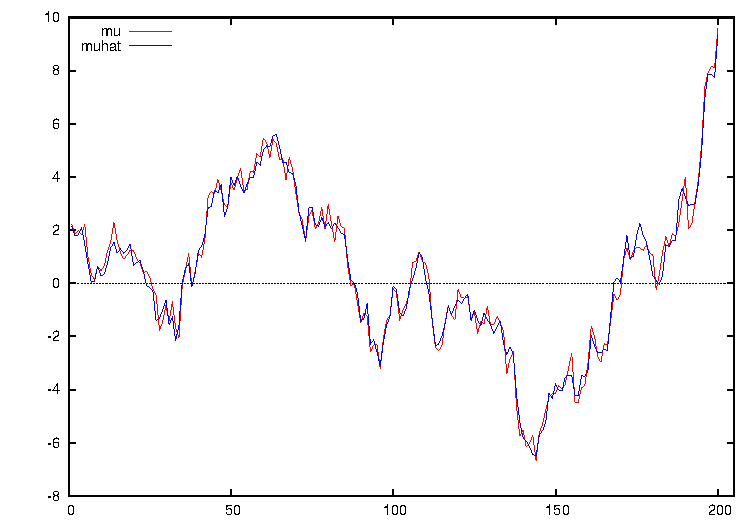
\includegraphics{figures/local_level}
%   \caption{Local level model: $\mu_t$ and its smoothed estimate}
%   \label{fig:loclev}
% \end{figure}

\begin{script}[htbp]
  \caption{Auxiliary residuals for the local level model --- Nile data}
  \label{script:auxres}
\begin{scode}
set echo off
set messages off

open nile.gdt

# ML estimates
scalar s2_eta = 1468.49
scalar s2_eps = 15099.7

bundle LLM = ksetup(nile, 1, 1, s2_eta)
LLM.obsvar = s2_eps
LLM.diffuse = 1

kdsmooth(&LLM)
series etahat = LLM.smdist[,1]
series var_etahat = LLM.stdistvar
series eta_aux = etahat/sqrt(var_etahat)
plot eta_aux
  options time-series with-lines
  literal set title 'Auxiliary residual, state equation'
  literal set ylabel ''
end plot --output=display

kdsmooth(&LLM, 1)
series sdeta = sqrt(LLM.stdistvar)
series eta_minus = etahat - 1.64485 * sdeta
series eta_plus = etahat + 1.64485 * sdeta
list P = etahat eta_minus eta_plus
plot P
  options time-series with-lines single-yaxis
  literal set linetype 3 lc rgb "#0000ff"
  literal set title 'State disturbance with 90% confidence band'
  literal set nokey
end plot --output=display  
\end{scode}
\end{script}


\section{Finer points}
\label{sec:finer}

\subsection{Cross-correlated disturbances}
\label{sec:crossd}

The formulation given in equations (\ref{eq:state}) and (\ref{eq:obs})
assumes mutual independence of the disturbances in the state and
observation equations, $\strdist_t$ and $\obsdist_t$.  This assumption
holds good in many practical applications, but a more general
formulation allows for cross-correlation.  In place of
(\ref{eq:state})--(\ref{eq:obs}) we may write
%
\begin{align*}
  \statevec_{t+1} &= \statemat_t \statevec_t + 
     \altstrvar_t \alldist_t \\
  \obsvec_t &= \obsxmat_t'\obsx_t + \obsmat_t' \statevec_t + 
     \altobsvar_t \alldist_t 
\end{align*}
%
where $\alldist_t$ is a ($p \times 1$) disturbance vector which is
assumed to satisfy $\alldist_t \sim N(0, I_p)$, $\altstrvar_t$ is
($r \times p$) and $\altobsvar_t$ is ($n \times p$).

In terms of input syntax, if the state and observation disturbances
are cross-correlated five arguments should be given to the
\cmd{ksetup} function (see section~\ref{sec:setup}): in place of
giving $\strvar$ you should give the two matrices identified above as
$\altstrvar$ and $\altobsvar$, as in
\begin{code}
bundle SSxmod = ksetup(y, H, F, B, C)
\end{code}

In case you wish to retrieve or update information on the variance of
the disturbances, note that in the cross-correlated case the bundle
keys \texttt{statevar} and \texttt{obsvar} are taken to designate the
factors $\altstrvar$ and $\altobsvar$ respectively.

\subsection{Constant term in the state equation}
\label{sec:stconst}

In some applications it is useful to be able to have a
constant term in the state transition equation, so as to generalize
equation \eqref{eq:state} to 
\[
  \statevec_{t+1} = \statemu + \statemat_t \statevec_t + \strdist_t \\
\]
The term $\statemu$ is never strictly necessary: the system
(\ref{eq:state}) and (\ref{eq:obs}) without $\statemu$ is general
enough to accommodate such a term, by absorbing it as an extra (non
time-varying) element in the state vector.  However, this comes at the
cost of expanding all the matrices that touch the state ($\statevec$,
$\statemat$, $\strdist$, $\strvar$, $\obsmat$), making the model
relatively awkward to formulate and forecasts more expensive to
compute. Therefore, we adopt the convention above on practical
grounds.

The ($r \times 1$) vector $\statemu$ can be specified as a bundle
member by the name \texttt{stconst}.

\subsection{Time-varying matrices}
\label{sec:tvarying}

Any or all of the matrices \texttt{obsymat}, \texttt{obsxmat},
\texttt{obsvar}, \texttt{statemat} and \texttt{statevar} may be
time-varying.  In that case you must supply the name of a function to
be called to update the matrix: you add this to the bundle as a
string, under a key which is composed of the keyword for the matrix in
question followed by an underscore and \texttt{call}.\footnote{The
  choice of the name for the function itself is of course totally up
  to the user.} For example, if \texttt{obsymat} ($\obsmat_t$) should
be updated by a function named \texttt{TV\_H} you would write
%
\begin{code}
SSmod.obsymat_call = "TV_H"
\end{code}
%
Functions that play this role will be called at each time-step of the
filter operation, prior to performing any calculations.  They should
take a single bundle-pointer argument; they will be passed a pointer
to the Kalman bundle to which the call is attached.  Such functions
have easy access to the following information from the bundle:
\begin{itemize}
\item The current time step (which starts at 1), under the
  reserved key \texttt{t}.
\item The $n$-vector containing the forecast error from the
  previous time step, $\prederr_{t-1}$, under the key \texttt{uhat};
  when $t=1$ this will be a zero vector.
\end{itemize}

If any additional information is needed for performing the update it
can be placed in the bundle under a user-specified key.  So, for
example, a simple updater for a $1 \times 1$ $\obsmat_t$ matrix might
look like this:
%
\begin{code}
function void TV_H (bundle *b)
    b.obsymat = b.Hvals[b.t]
end function
\end{code}
%
where the bundled matrix \texttt{b.Hvals} contains $T$ elements.

\subsection{Likelihood under the diffuse prior}
\label{sec:lldiffuse}

This note pertains to the \cmd{kfilter} function (see
section~\ref{sec:kfilter}). 

There seems to be general agreement in the literature that the
log-likelihood calculation should be modified in the case of a diffuse
prior for $\statevar_{1|0}$.  However, it is not clear to us that
there is a well-defined ``correct'' method for this.  At present we
emulate \textsf{SsfPack}.  In case
$\statevar_{1|0} = \kappa \mathbf{I}_r$, we set $d = r$ and calculate
%
\[
  \ell = -\frac{1}{2} \left[(nT-d) \log(2 \pi) + 
    \sum_{t=1}^T\log \left|\predvar_t\right| + 
    \sum_{t=1}^T\prederr_t'\predvar_t^{-1} \prederr_t
    - d \log(\kappa)
  \right]
\]
%
and
%
\[
\hat{\sigma}^2 = \frac{1}{nT-d} 
   \sum_{t=1}^T\prederr_t'\predvar_t^{-1} \prederr_t
\]
 

\end{document}
